

\chapter{Errores}

Las mediciones no son exactas, ya que, suponiendo que no exista ningún error humano en el proceso de medición, dependen de la precisión del instrumento. En otras palabras, toda medida estará afectada por un error.

\subsection{Error absoluto}
Si se supone una medida $X_v$ teórica ideal exacta y $X_m$ el valor medido real, el error absoluto $E_{abs}$ se define como la diferencia entre ambos: $$ E_{abs}= X_m-X_v $$

\subsection{Tolerancia}
En la mayoría de los casos, es posible calcular el mayor error absoluto posible (límite de error) en una medición, recurriendo al análisis de las características de los instrumentos y de las técnicas utilizadas. Así, se podría expresar una medición con su respectiva tolerancia, para indicar el grado de precisión de dicha medida.

\begin{ejemplo}
	Un capacitor posee una capacidad de $10 \mu F \pm 0,1 \mu F$. Esto significa que su valor real estará comprendido entre $10,1 \mu F$ y $9,9 \mu F$.
\end{ejemplo}

\begin{ejemplo}
	Un resistor posee una resistencia de $1000 \Omega \pm 5 \% $. Esto significa que su valor real estará comprendido entre $ 950 \Omega $ y $ 1050 \Omega $.
\end{ejemplo}

\subsubsection{Valor verdadero probable}
Debido a que se desconoce el valor verdadero original, se tomará el valor verdadero probable $X_v'$, que considerará todas las causas de error posibles (por el operador, por el método y por el instrumento utilizado).

De ese modo, se puede redefinir el error absoluto como: $$ E_{abs}= X_m-X_v' $$

\subsection{Error relativo}

El error relativo permite conocer la magnitud de un error cometido. Se calcula efectuando el cociente entre el error absoluto y el valor real.

$$ E_{rel} = \frac{X_m-X_v'}{X_v'} $$

\subsubsection{Error relativo porcentual}

Suele ser útil expresar el error relativo como porcentaje. Para eso, multiplicamos el error relativo $E_{rel}$ por $100$: $$ e\% = 100 \times E_{rel} $$

\begin{ejemplo} \label{ejE:1}
	Se tomó la medición de la tensión de una rama de un circuito, obteniendo un valor de $30 V$, y un valor real de $27 V$.
	
	Hallar el error absoluto, el error relativo y el error relativo porcentual.
	
	\emph{Solución:} $$ E_{abs}= 30 V-27 V = 3 V $$ 
	$$ E_{rel} = \frac{3 V}{27 V} \approx 0,1111 V$$
	$$ e\% = 100 \times 0,1111 V = 11,11 \% $$
\end{ejemplo}

\begin{ejemplo}
	\label{ejE:2}
	Se tomó la medición de la tensión de una rama de un circuito, obteniendo un valor de $233 V$, y un valor real de $230 V$.
	
	Hallar el error absoluto, el error relativo y el error relativo porcentual.
	
	\emph{Solución:} $$ E_{abs}= 233 V- 230 V = 3 V $$ 
	$$ E_{rel} = \frac{3 V}{230 V} \approx 0,01304 V$$
	$$ e\% = 100 \times 0,01304 V = 1,3 \% $$
\end{ejemplo}

Nótese que, si bien en ambos ejemplos el error absoluto es el mismo, el error relativo del ejemplo \ref{ejE:1} es mucho mayor que la del ejemplo \ref{ejE:2}; por lo que la segunda medición es mucho más precisa.

\section{Clasificación de los errores}
\subsection{Errores groseros}
Son los errores producidos por una mala elección del instrumento o del método, por una mala interpretación del operario (como por ejemplo una transposición de cifras), o bien por una implementación errónea (una lectura en escala incorrecta).

Es posible detectar errores groseros controlando de forma permanente la coherencia de los valores dentro de una serie de mediciones. Si existe un valor que resulte sospechoso para el contexto en el cual se tomó, entonces debería revisarse.

\subsection{Errores sistemáticos}

Son errores que se producen en todas las mediciones tomadas.

Pueden producirse por:
\begin{itemize}
	\item Errores en el método utilizado.
	\item Errores en los instrumentos, ya sea por la clase de los mismos como por el desgaste natural o el uso en condiciones inadecuadas.
	\item Errores por tendencia del observador, ya sea en exceso o en defecto.
	\item Errores condicionados por el ambiente. Aspectos como la temperatura, humedad, vibraciones o presión, pueden afectar la precisión de un instrumento o de la técnica utilizada.
\end{itemize}
\section{Clase de un instrumento}
La clase de un instrumento es uno de los indicadores de la precisión del mismo. Es el valor porcentual que expresa la relación entre el error absoluto y el alcance del mismo:

$$ Clase = \frac{E_{abs}max}{Alcance}\times 100 $$
\begin{figure}
	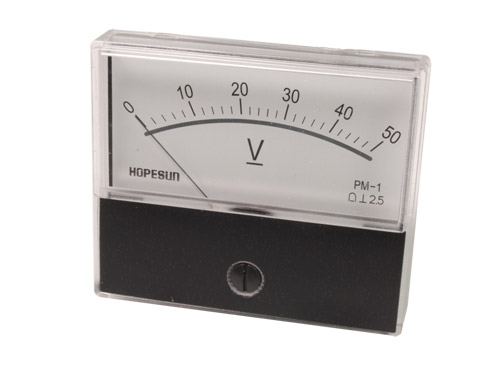
\includegraphics[scale=0.7]{images/volt_clase}
	\caption{Voltímetro Clase 2,5}
	\label{fig:voltclase}
\end{figure}
\begin{ejemplo}
	En la figura \ref{fig:voltclase}, se puede apreciar que la clase del instrumento es 2,5. Como se ve, el alcance máximo es de 50 V. ¿Cuál es el error absoluto máximo que puede producirse?
	
	\emph{Solución:} Reemplazando en la ecuación de clase:
	
	$$ 2,5 = \frac{ErrorAbsMax}{50 V} \times 100 
	\rightarrow
	ErrorAbsMax = \frac{2,5 \times 50V}{100} = 1,25 V $$
	
	
\end{ejemplo}

\begin{tabular}{|c|c|}
\hline 
Clase del instrumento & Aplicación \\ 
\hline 
0.05 a 0.1 & Patrones de referencia. Calibración de instrumentos. Ensayos de laboratorio muy precisos. \\ 
\hline 
0.2 a 0.5 & Ensayos de laboratorio. Contraste de instrumentos de una clase al menos 5 veces mayor \\ 
\hline 
>1 & Tableros, paneles de escala vertical, instrumentos portátiles de baja precisión. \\ 
\hline 
\end{tabular} 